\documentclass[11pt]{article}
\usepackage[textwidth=18.0cm, textheight=23.0cm, top=2.0cm]{geometry}
\usepackage{pst-all}
\usepackage{amssymb}
\usepackage{tikz}
\usepackage{underscore}\begin{document}
\pagestyle{empty}


ClassName: \underline{\textbf{Class_03.2bp-24}}
\par
BinSize: \underline{\textbf{40 × 40}}
\par
ReduceSize: \underline{\textbf{40 × 40}}
\par
TypeNum: \underline{\textbf{60}}
\par
Num: \underline{\textbf{60}}
\par
OutS: \underline{\textbf{19200}}
\par
InS: \underline{\textbf{17407}}
\par
Rate: \underline{\textbf{0.907}}
\par
UB: \underline{\textbf{12}}
\par
LB0: \underline{\textbf{12}}
\par
LB: \underline{\textbf{12}}
\par
LBWithCut: \underline{\textbf{12}}
\par
NodeCut: \underline{\textbf{0}}
\par
ExtendedNodeCnt: \underline{\textbf{1}}
\par
GenNodeCnt: \underline{\textbf{1}}
\par
PrimalNode: \underline{\textbf{0}}
\par
ColumnCount: \underline{\textbf{12}}
\par
TotalCutCount: \underline{\textbf{0}}
\par
RootCutCount: \underline{\textbf{0}}
\par
LPSolverCnt: \underline{\textbf{1}}
\par
PricingSolverCnt: \underline{\textbf{0}}
\par
BranchAndBoundNum: \underline{\textbf{1}}
\par
isOpt: \underline{\textbf{true}}
\par
TimeOnPrimal: \underline{\textbf{0.000 s}}
\par
TimeOnPricing: \underline{\textbf{0.000 s}}
\par
TimeOnRmp: \underline{\textbf{0.078 s}}
\par
TotalTime: \underline{\textbf{0.140 s}}
\par
\newpage


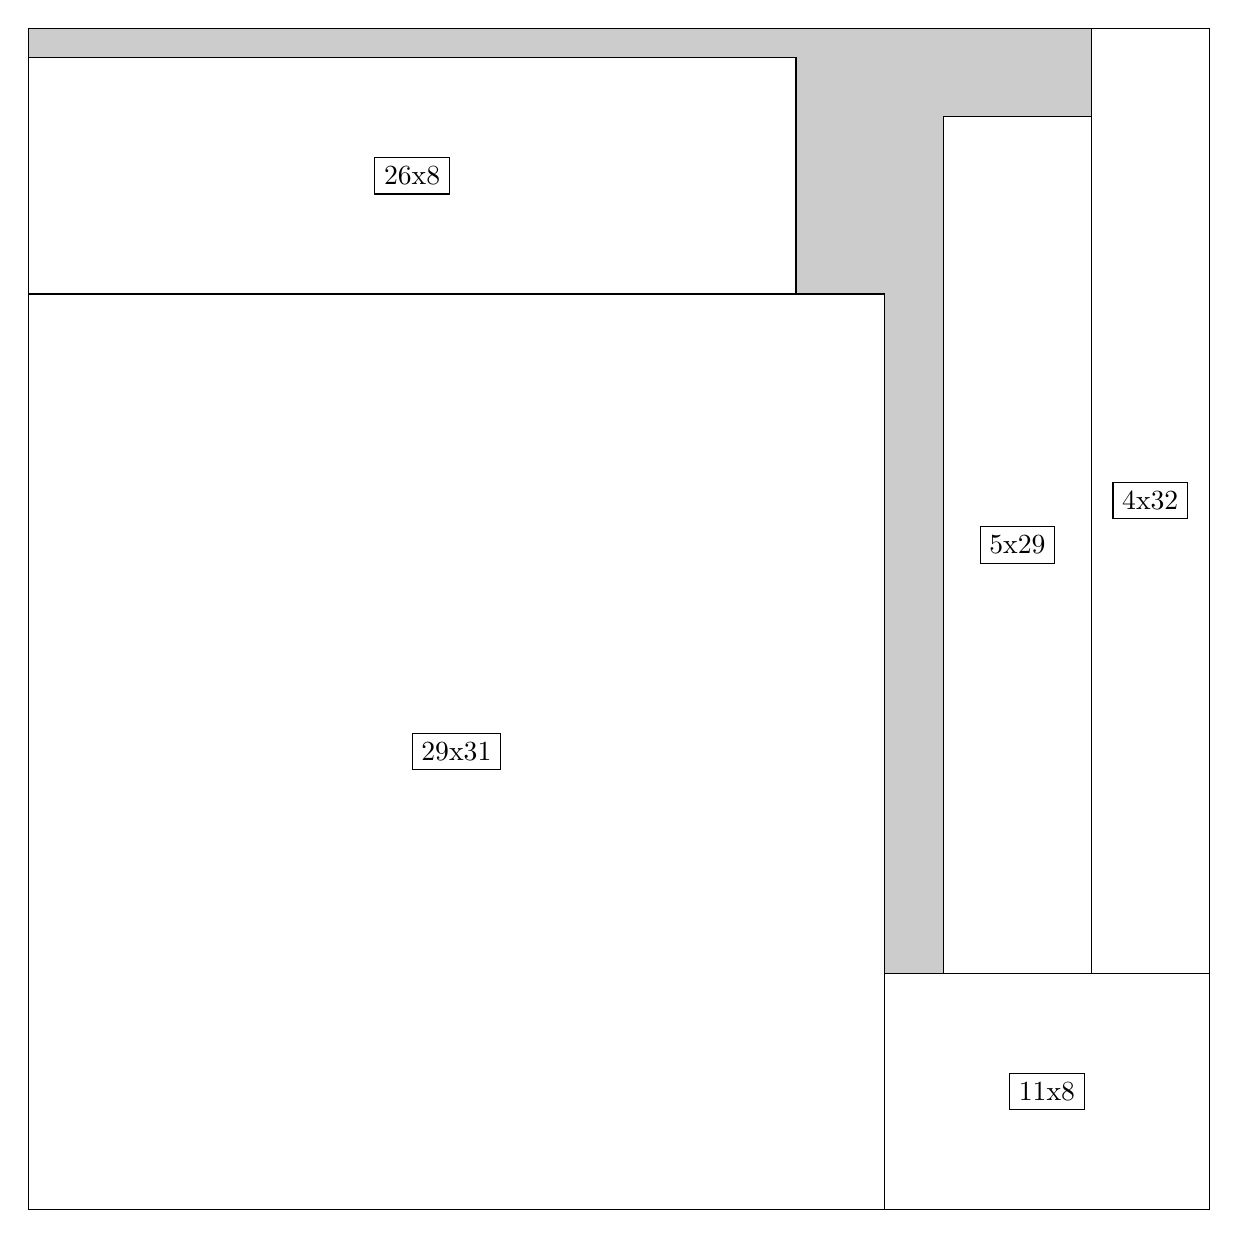
\begin{tikzpicture}[shorten >=1pt,scale=1.0,every node/.style={scale=1.0},->]
\tikzstyle{vertex}=[circle,fill=black!25,minimum size=14pt,inner sep=0pt]
\filldraw[fill=gray!40!white, draw=black] (0,0) rectangle (15.0,15.0);
\foreach \name/\x/\y/\w/\h in {29x31/0.0/0.0/10.875/11.625,26x8/0.0/11.625/9.75/3.0,5x29/11.625/3.0/1.875/10.875,4x32/13.5/3.0/1.5/12.0,11x8/10.875/0.0/4.125/3.0}
\filldraw[fill=white!40!white, draw=black] (\x,\y) rectangle node[draw] (\name) {\name} ++(\w,\h);
\end{tikzpicture}


w =29 , h =31 , x =0 , y =0 , v =899
\par
w =26 , h =8 , x =0 , y =31 , v =208
\par
w =5 , h =29 , x =31 , y =8 , v =145
\par
w =4 , h =32 , x =36 , y =8 , v =128
\par
w =11 , h =8 , x =29 , y =0 , v =88
\par
\newpage


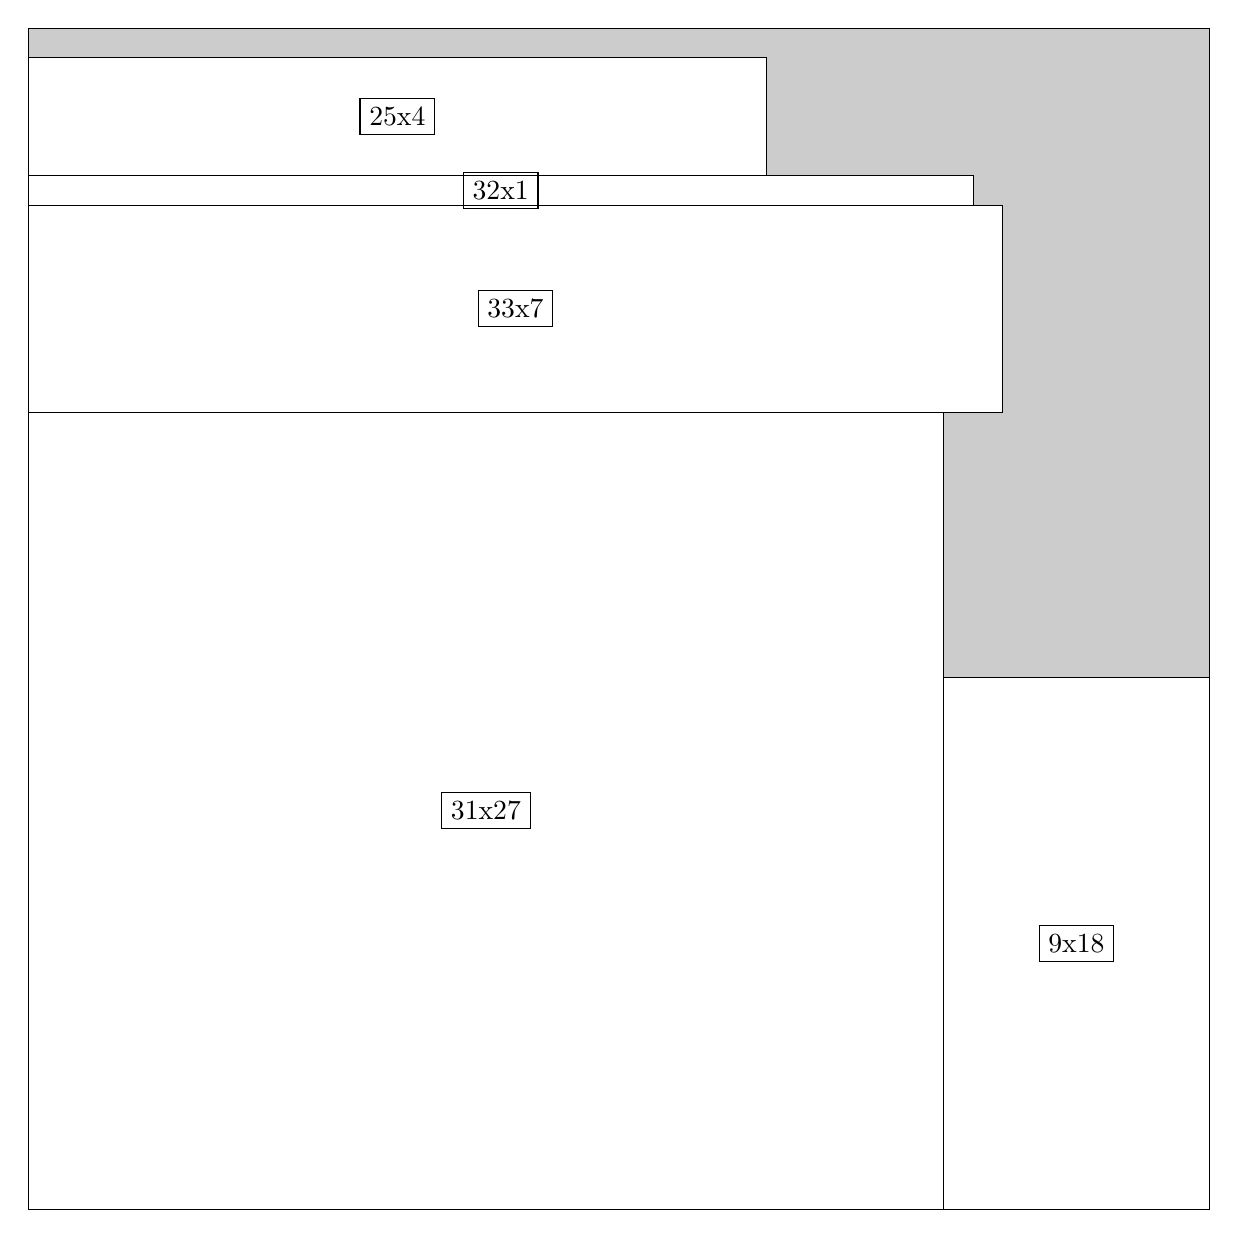
\begin{tikzpicture}[shorten >=1pt,scale=1.0,every node/.style={scale=1.0},->]
\tikzstyle{vertex}=[circle,fill=black!25,minimum size=14pt,inner sep=0pt]
\filldraw[fill=gray!40!white, draw=black] (0,0) rectangle (15.0,15.0);
\foreach \name/\x/\y/\w/\h in {31x27/0.0/0.0/11.625/10.125,33x7/0.0/10.125/12.375/2.625,9x18/11.625/0.0/3.375/6.75,25x4/0.0/13.125/9.375/1.5,32x1/0.0/12.75/12.0/0.375}
\filldraw[fill=white!40!white, draw=black] (\x,\y) rectangle node[draw] (\name) {\name} ++(\w,\h);
\end{tikzpicture}


w =31 , h =27 , x =0 , y =0 , v =837
\par
w =33 , h =7 , x =0 , y =27 , v =231
\par
w =9 , h =18 , x =31 , y =0 , v =162
\par
w =25 , h =4 , x =0 , y =35 , v =100
\par
w =32 , h =1 , x =0 , y =34 , v =32
\par
\newpage


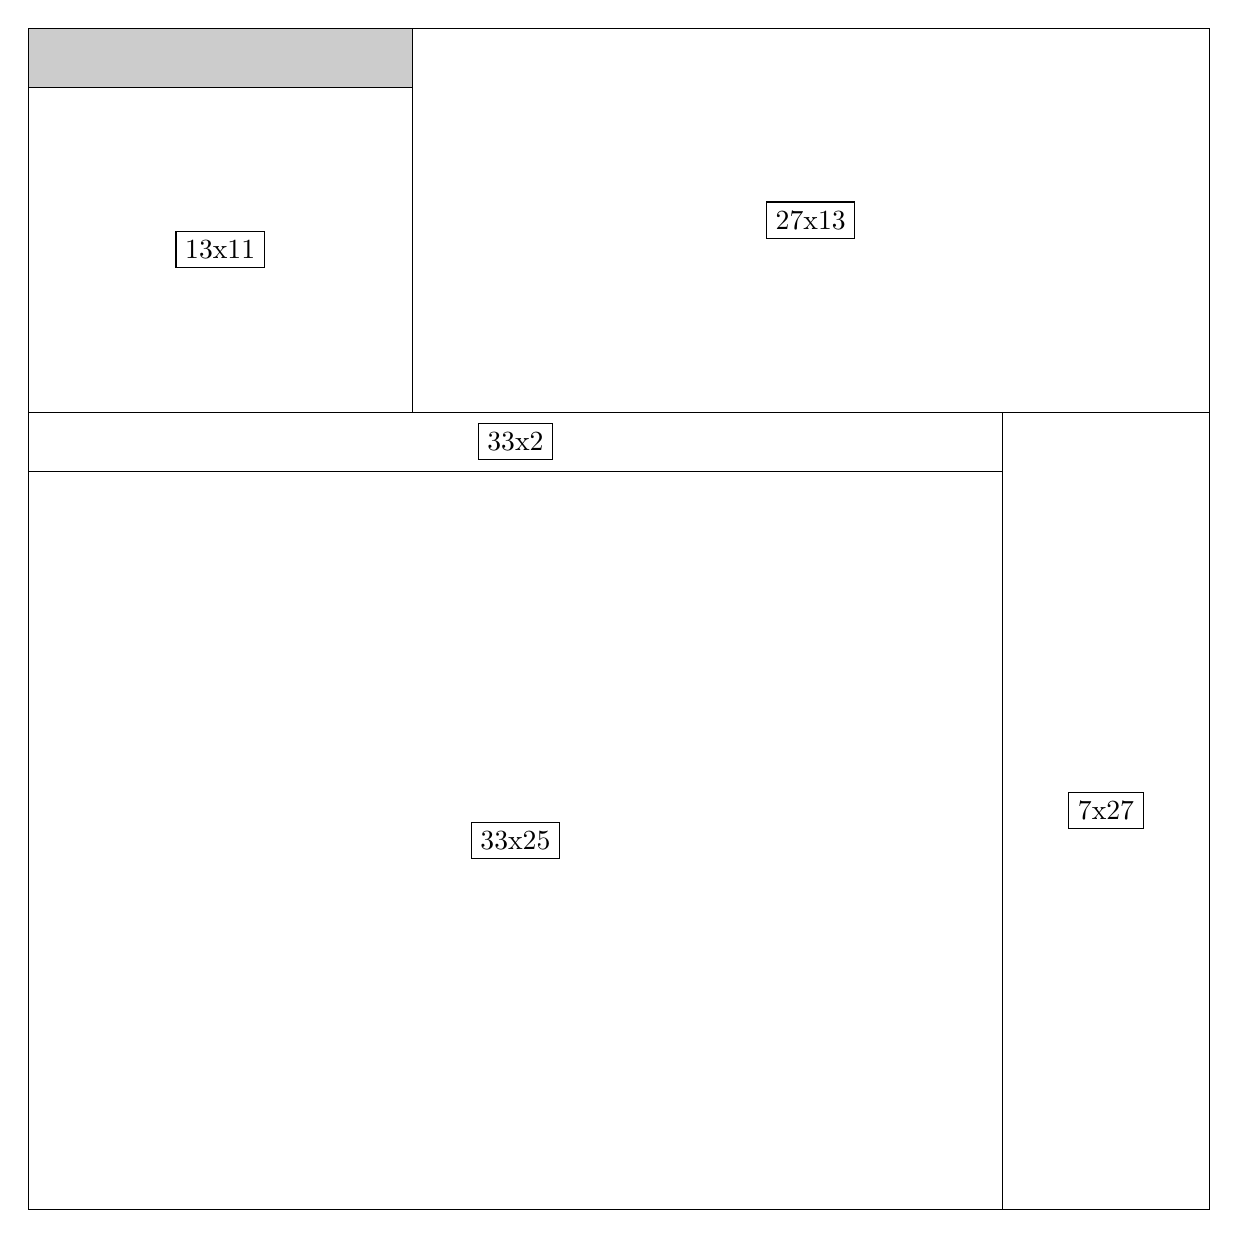
\begin{tikzpicture}[shorten >=1pt,scale=1.0,every node/.style={scale=1.0},->]
\tikzstyle{vertex}=[circle,fill=black!25,minimum size=14pt,inner sep=0pt]
\filldraw[fill=gray!40!white, draw=black] (0,0) rectangle (15.0,15.0);
\foreach \name/\x/\y/\w/\h in {33x25/0.0/0.0/12.375/9.375,27x13/4.875/10.125/10.125/4.875,7x27/12.375/0.0/2.625/10.125,13x11/0.0/10.125/4.875/4.125,33x2/0.0/9.375/12.375/0.75}
\filldraw[fill=white!40!white, draw=black] (\x,\y) rectangle node[draw] (\name) {\name} ++(\w,\h);
\end{tikzpicture}


w =33 , h =25 , x =0 , y =0 , v =825
\par
w =27 , h =13 , x =13 , y =27 , v =351
\par
w =7 , h =27 , x =33 , y =0 , v =189
\par
w =13 , h =11 , x =0 , y =27 , v =143
\par
w =33 , h =2 , x =0 , y =25 , v =66
\par
\newpage


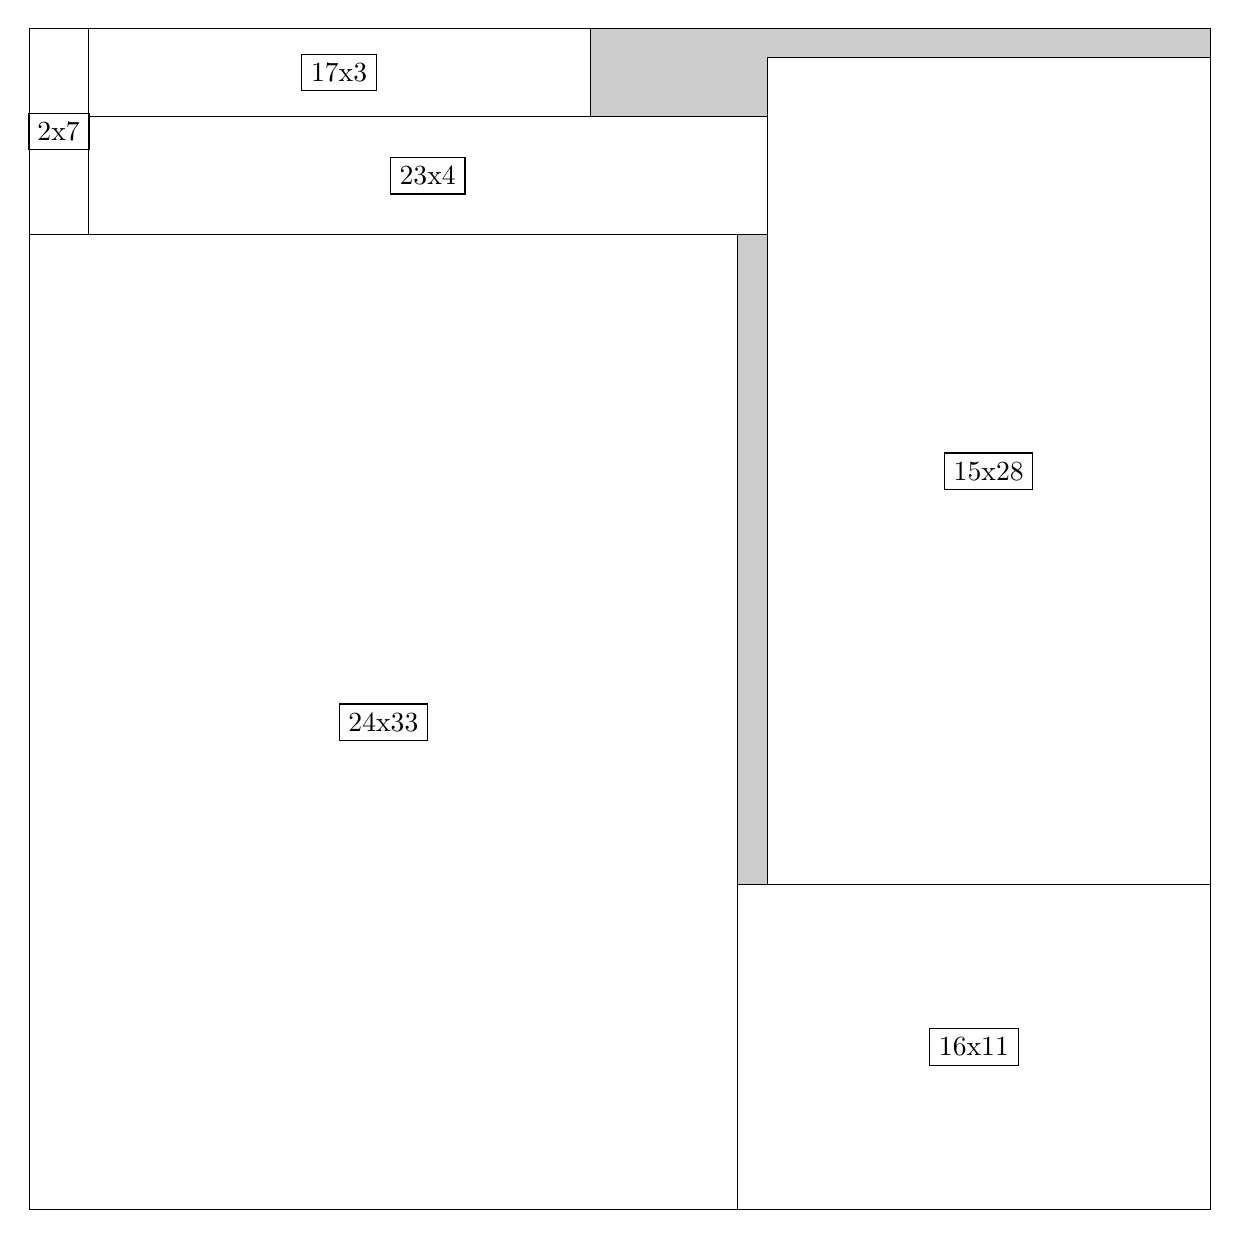
\begin{tikzpicture}[shorten >=1pt,scale=1.0,every node/.style={scale=1.0},->]
\tikzstyle{vertex}=[circle,fill=black!25,minimum size=14pt,inner sep=0pt]
\filldraw[fill=gray!40!white, draw=black] (0,0) rectangle (15.0,15.0);
\foreach \name/\x/\y/\w/\h in {24x33/0.0/0.0/9.0/12.375,15x28/9.375/4.125/5.625/10.5,23x4/0.75/12.375/8.625/1.5,17x3/0.75/13.875/6.375/1.125,16x11/9.0/0.0/6.0/4.125,2x7/0.0/12.375/0.75/2.625}
\filldraw[fill=white!40!white, draw=black] (\x,\y) rectangle node[draw] (\name) {\name} ++(\w,\h);
\end{tikzpicture}


w =24 , h =33 , x =0 , y =0 , v =792
\par
w =15 , h =28 , x =25 , y =11 , v =420
\par
w =23 , h =4 , x =2 , y =33 , v =92
\par
w =17 , h =3 , x =2 , y =37 , v =51
\par
w =16 , h =11 , x =24 , y =0 , v =176
\par
w =2 , h =7 , x =0 , y =33 , v =14
\par
\newpage


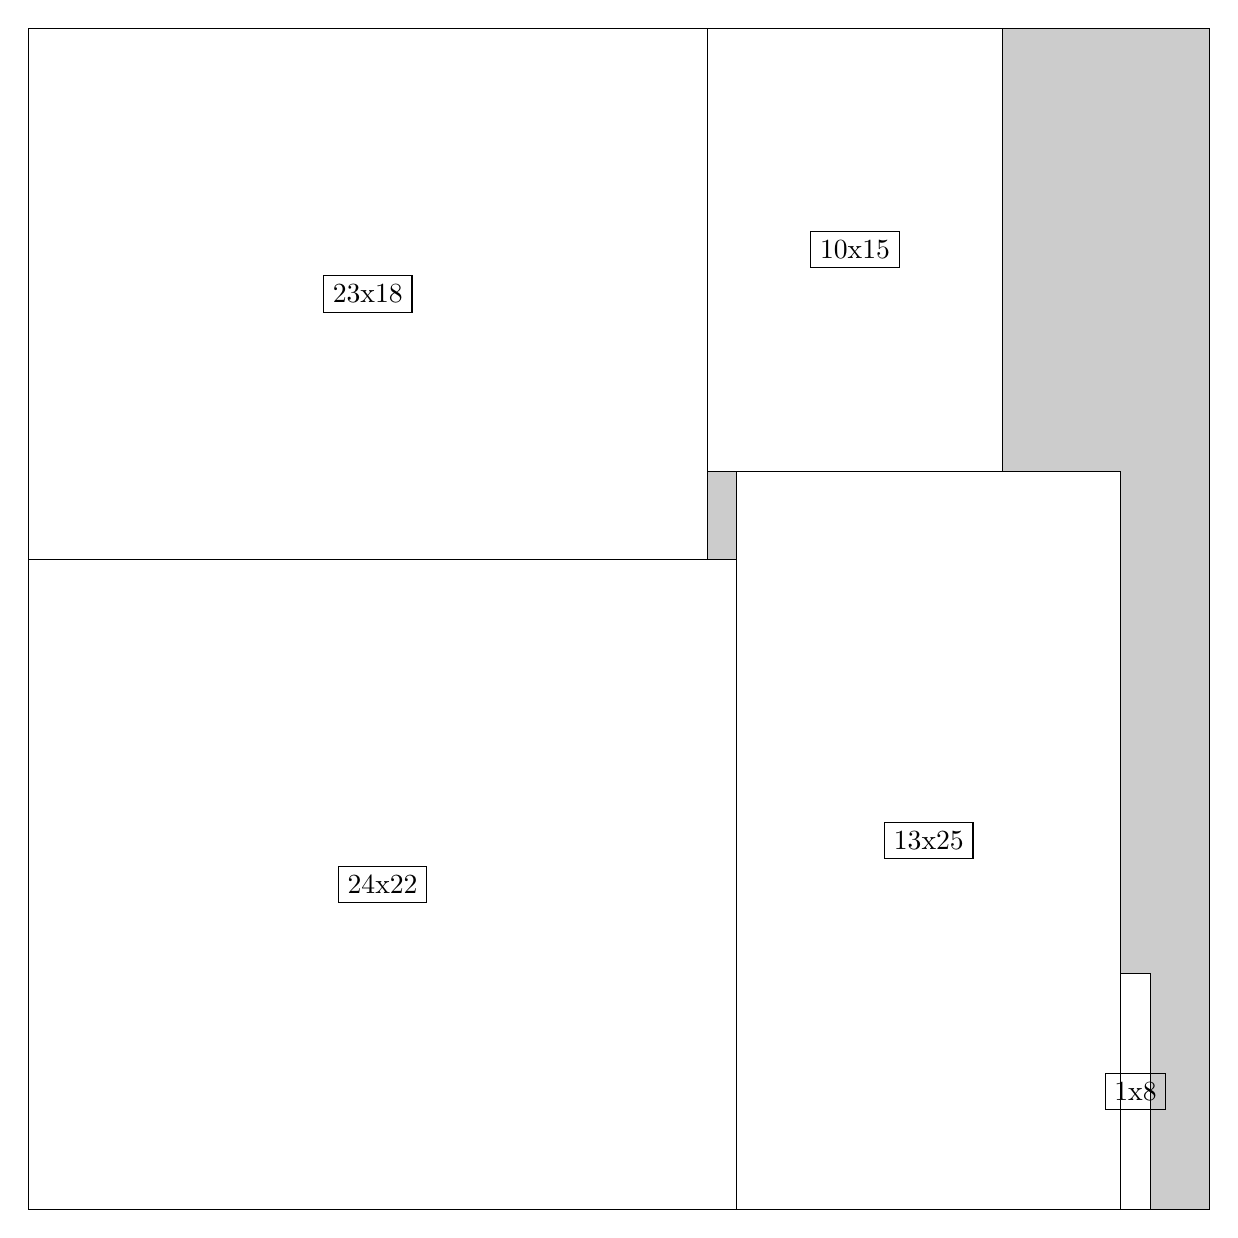
\begin{tikzpicture}[shorten >=1pt,scale=1.0,every node/.style={scale=1.0},->]
\tikzstyle{vertex}=[circle,fill=black!25,minimum size=14pt,inner sep=0pt]
\filldraw[fill=gray!40!white, draw=black] (0,0) rectangle (15.0,15.0);
\foreach \name/\x/\y/\w/\h in {24x22/0.0/0.0/9.0/8.25,23x18/0.0/8.25/8.625/6.75,13x25/9.0/0.0/4.875/9.375,10x15/8.625/9.375/3.75/5.625,1x8/13.875/0.0/0.375/3.0}
\filldraw[fill=white!40!white, draw=black] (\x,\y) rectangle node[draw] (\name) {\name} ++(\w,\h);
\end{tikzpicture}


w =24 , h =22 , x =0 , y =0 , v =528
\par
w =23 , h =18 , x =0 , y =22 , v =414
\par
w =13 , h =25 , x =24 , y =0 , v =325
\par
w =10 , h =15 , x =23 , y =25 , v =150
\par
w =1 , h =8 , x =37 , y =0 , v =8
\par
\newpage


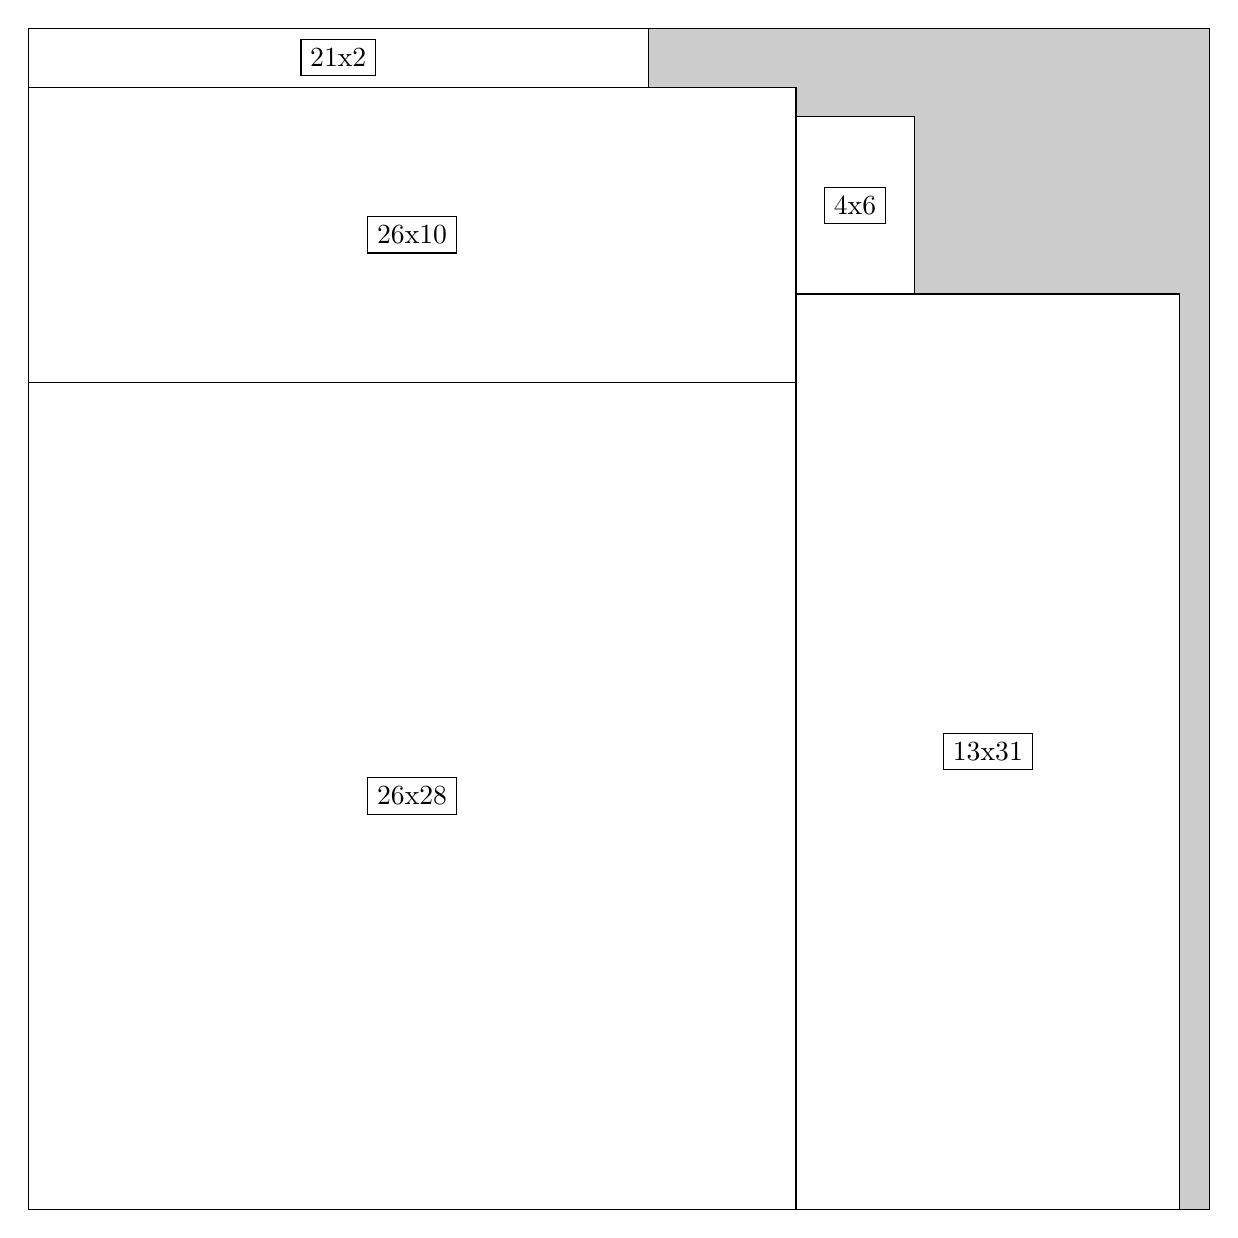
\begin{tikzpicture}[shorten >=1pt,scale=1.0,every node/.style={scale=1.0},->]
\tikzstyle{vertex}=[circle,fill=black!25,minimum size=14pt,inner sep=0pt]
\filldraw[fill=gray!40!white, draw=black] (0,0) rectangle (15.0,15.0);
\foreach \name/\x/\y/\w/\h in {26x28/0.0/0.0/9.75/10.5,13x31/9.75/0.0/4.875/11.625,26x10/0.0/10.5/9.75/3.75,4x6/9.75/11.625/1.5/2.25,21x2/0.0/14.25/7.875/0.75}
\filldraw[fill=white!40!white, draw=black] (\x,\y) rectangle node[draw] (\name) {\name} ++(\w,\h);
\end{tikzpicture}


w =26 , h =28 , x =0 , y =0 , v =728
\par
w =13 , h =31 , x =26 , y =0 , v =403
\par
w =26 , h =10 , x =0 , y =28 , v =260
\par
w =4 , h =6 , x =26 , y =31 , v =24
\par
w =21 , h =2 , x =0 , y =38 , v =42
\par
\newpage


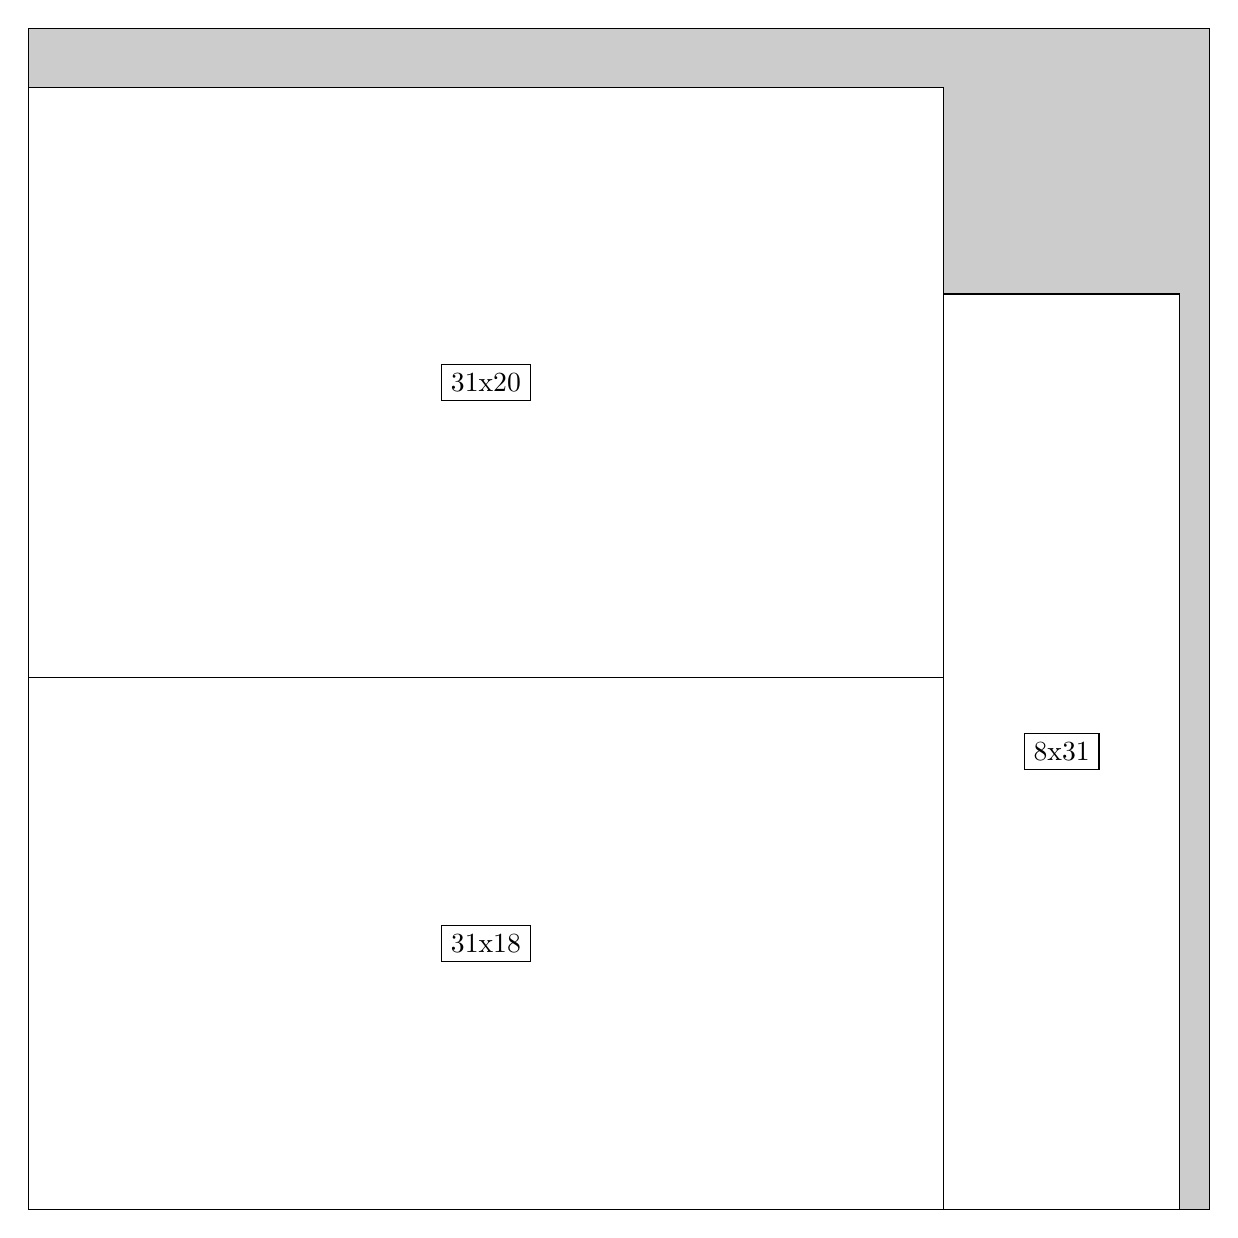
\begin{tikzpicture}[shorten >=1pt,scale=1.0,every node/.style={scale=1.0},->]
\tikzstyle{vertex}=[circle,fill=black!25,minimum size=14pt,inner sep=0pt]
\filldraw[fill=gray!40!white, draw=black] (0,0) rectangle (15.0,15.0);
\foreach \name/\x/\y/\w/\h in {31x18/0.0/0.0/11.625/6.75,31x20/0.0/6.75/11.625/7.5,8x31/11.625/0.0/3.0/11.625}
\filldraw[fill=white!40!white, draw=black] (\x,\y) rectangle node[draw] (\name) {\name} ++(\w,\h);
\end{tikzpicture}


w =31 , h =18 , x =0 , y =0 , v =558
\par
w =31 , h =20 , x =0 , y =18 , v =620
\par
w =8 , h =31 , x =31 , y =0 , v =248
\par
\newpage


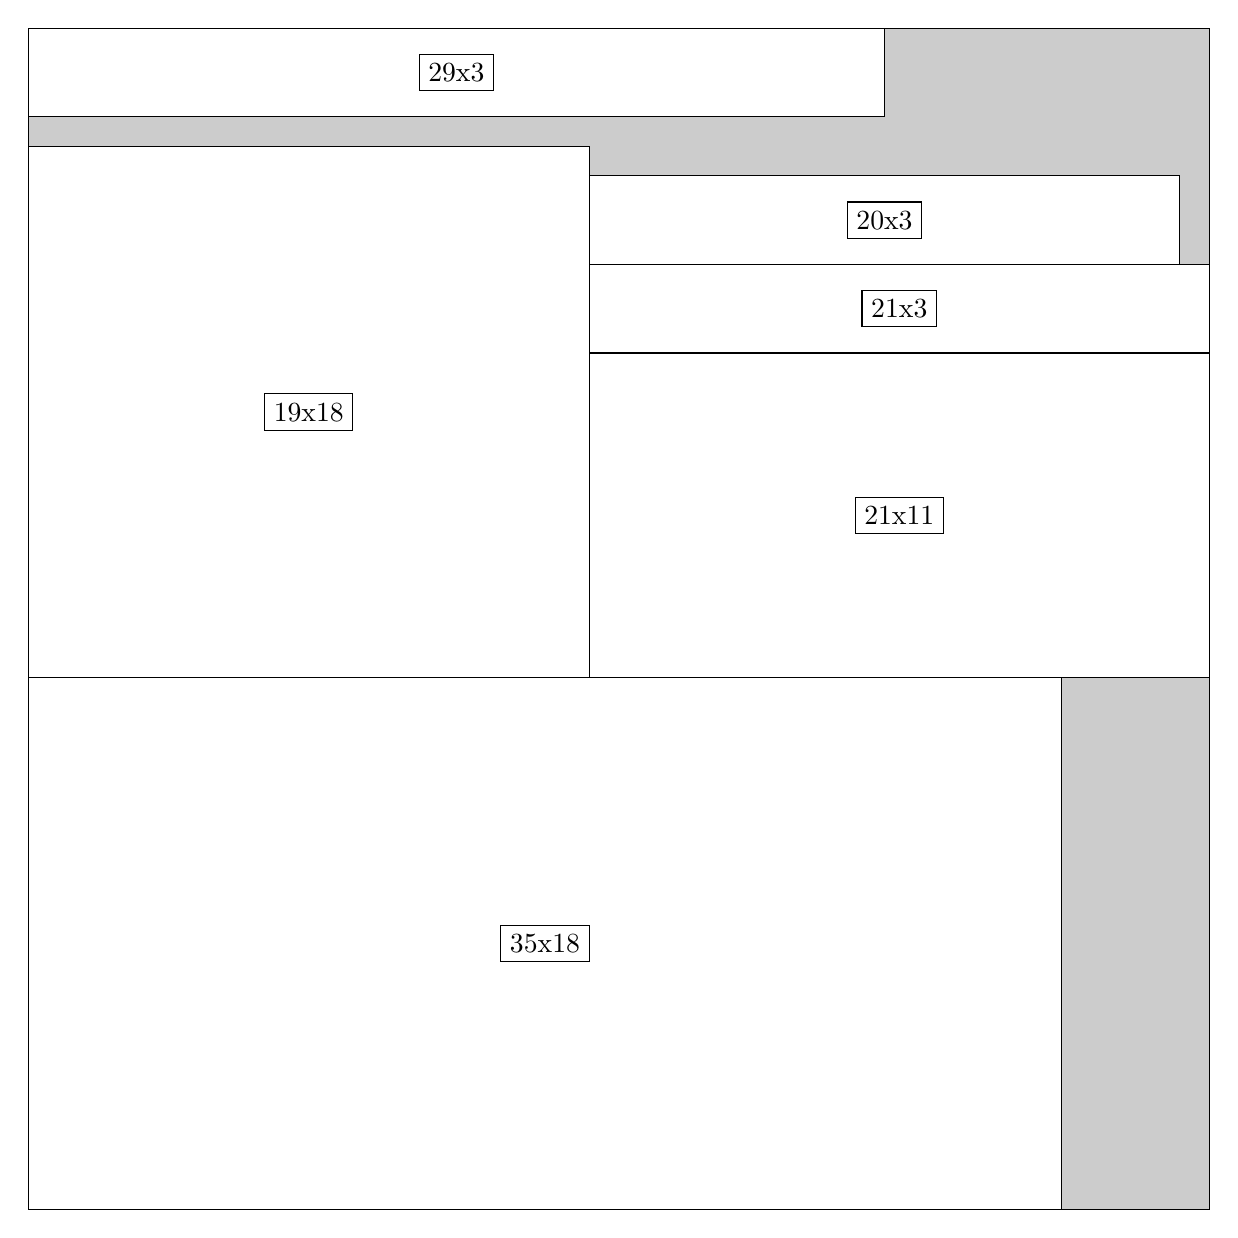
\begin{tikzpicture}[shorten >=1pt,scale=1.0,every node/.style={scale=1.0},->]
\tikzstyle{vertex}=[circle,fill=black!25,minimum size=14pt,inner sep=0pt]
\filldraw[fill=gray!40!white, draw=black] (0,0) rectangle (15.0,15.0);
\foreach \name/\x/\y/\w/\h in {35x18/0.0/0.0/13.125/6.75,19x18/0.0/6.75/7.125/6.75,21x11/7.125/6.75/7.875/4.125,29x3/0.0/13.875/10.875/1.125,21x3/7.125/10.875/7.875/1.125,20x3/7.125/12.0/7.5/1.125}
\filldraw[fill=white!40!white, draw=black] (\x,\y) rectangle node[draw] (\name) {\name} ++(\w,\h);
\end{tikzpicture}


w =35 , h =18 , x =0 , y =0 , v =630
\par
w =19 , h =18 , x =0 , y =18 , v =342
\par
w =21 , h =11 , x =19 , y =18 , v =231
\par
w =29 , h =3 , x =0 , y =37 , v =87
\par
w =21 , h =3 , x =19 , y =29 , v =63
\par
w =20 , h =3 , x =19 , y =32 , v =60
\par
\newpage


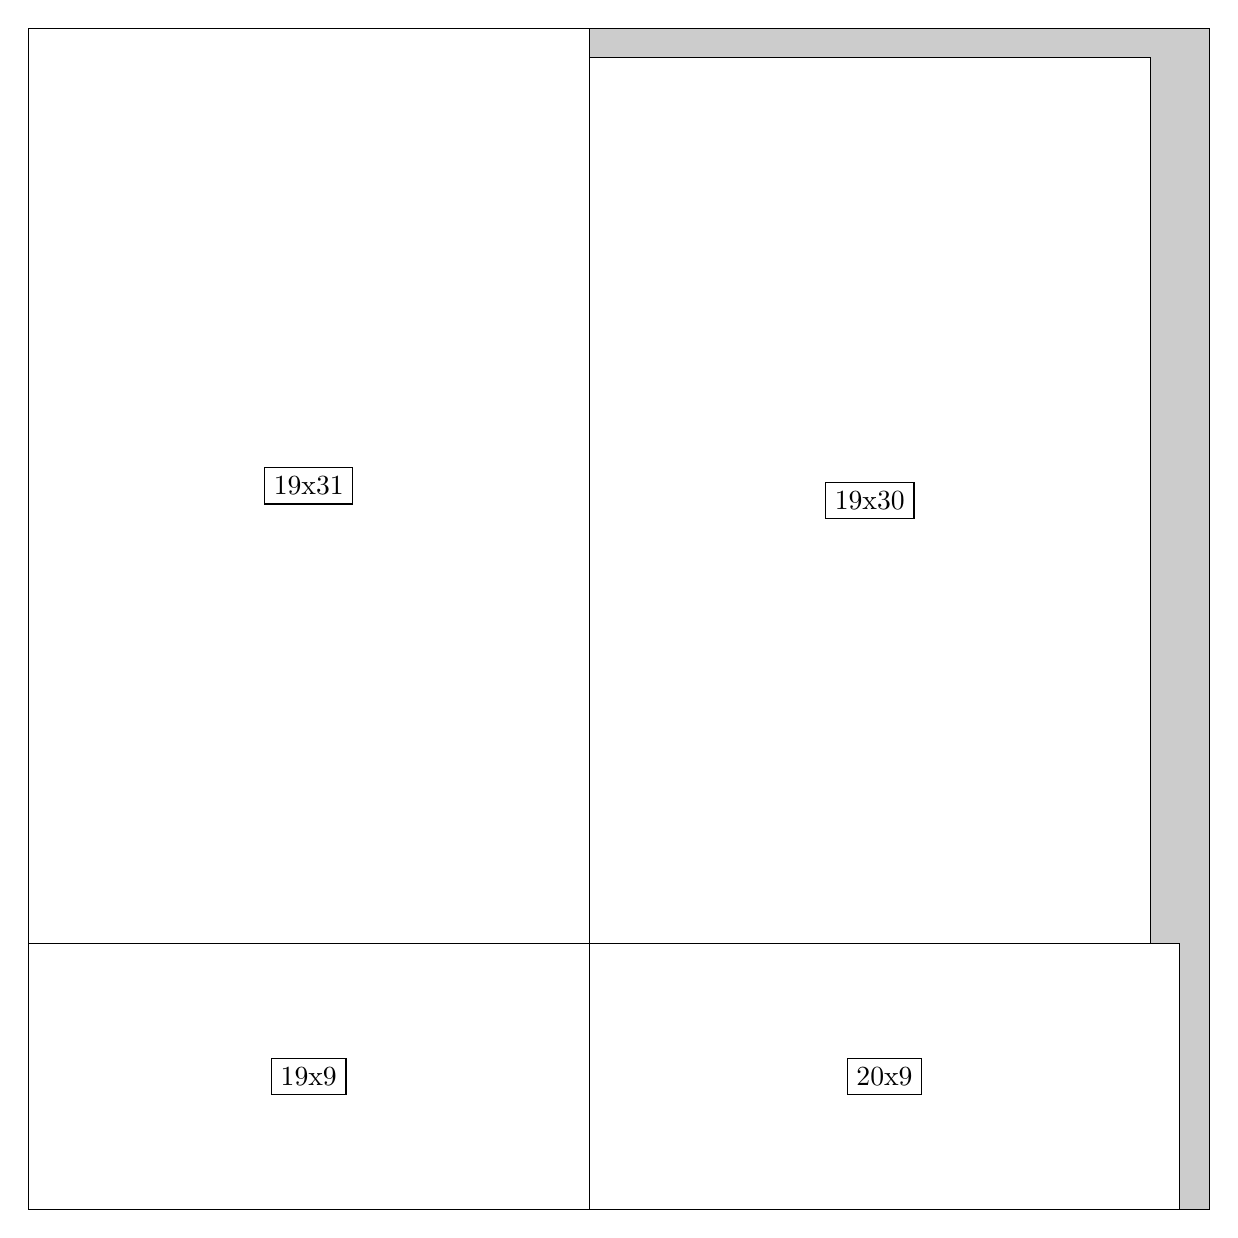
\begin{tikzpicture}[shorten >=1pt,scale=1.0,every node/.style={scale=1.0},->]
\tikzstyle{vertex}=[circle,fill=black!25,minimum size=14pt,inner sep=0pt]
\filldraw[fill=gray!40!white, draw=black] (0,0) rectangle (15.0,15.0);
\foreach \name/\x/\y/\w/\h in {19x9/0.0/0.0/7.125/3.375,19x31/0.0/3.375/7.125/11.625,19x30/7.125/3.375/7.125/11.25,20x9/7.125/0.0/7.5/3.375}
\filldraw[fill=white!40!white, draw=black] (\x,\y) rectangle node[draw] (\name) {\name} ++(\w,\h);
\end{tikzpicture}


w =19 , h =9 , x =0 , y =0 , v =171
\par
w =19 , h =31 , x =0 , y =9 , v =589
\par
w =19 , h =30 , x =19 , y =9 , v =570
\par
w =20 , h =9 , x =19 , y =0 , v =180
\par
\newpage


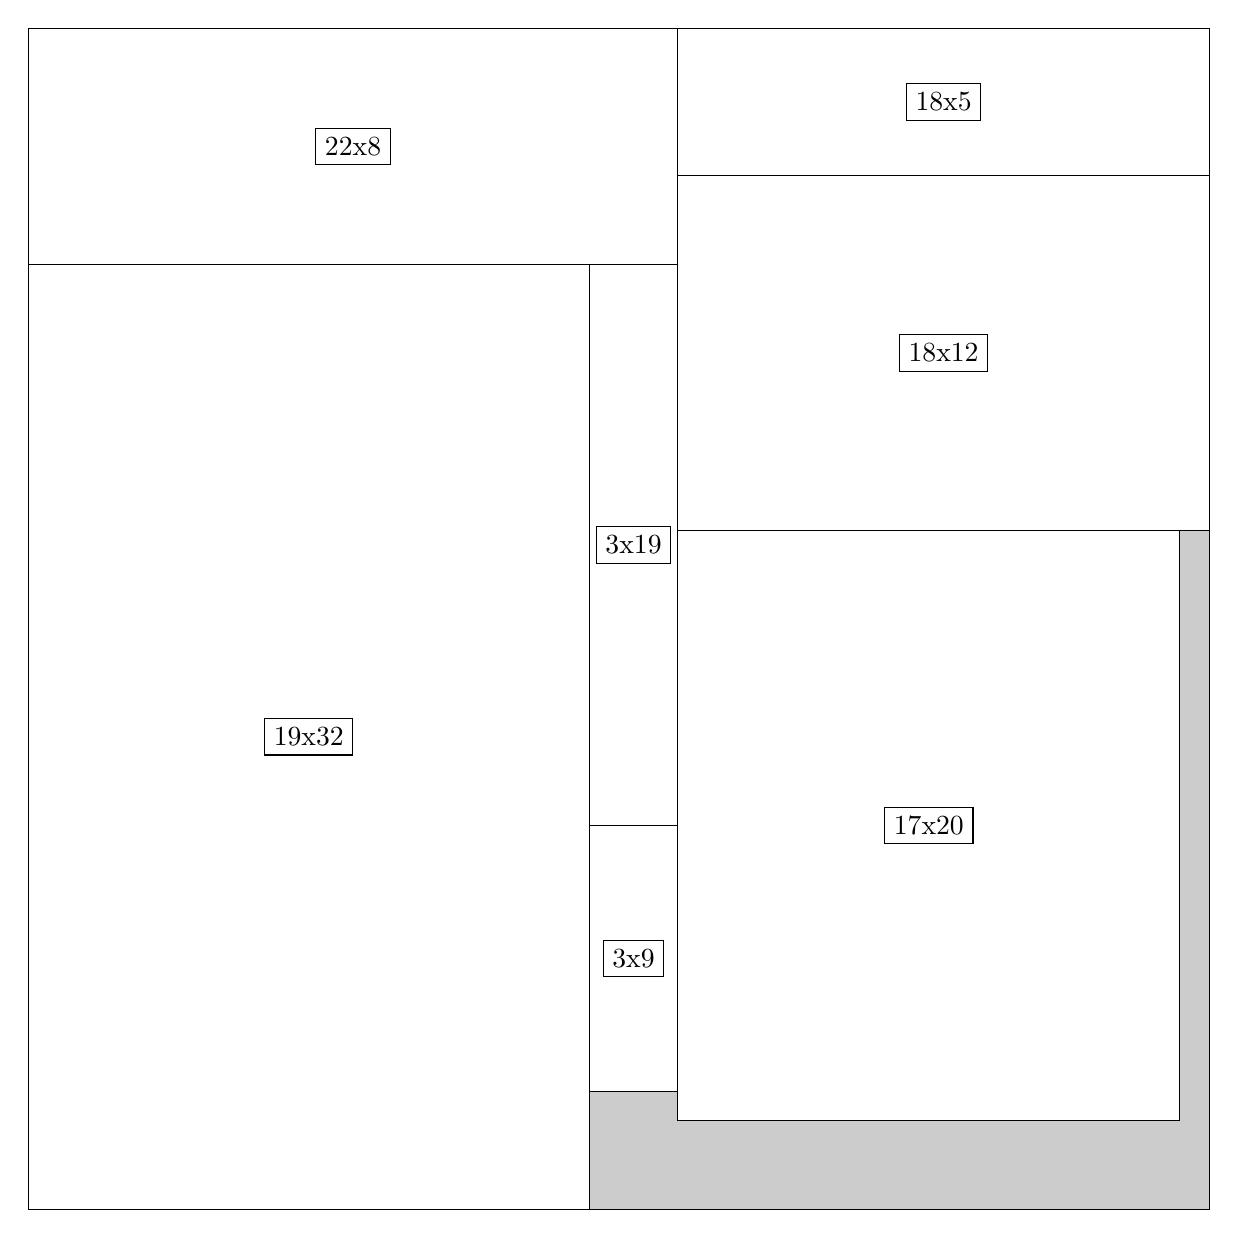
\begin{tikzpicture}[shorten >=1pt,scale=1.0,every node/.style={scale=1.0},->]
\tikzstyle{vertex}=[circle,fill=black!25,minimum size=14pt,inner sep=0pt]
\filldraw[fill=gray!40!white, draw=black] (0,0) rectangle (15.0,15.0);
\foreach \name/\x/\y/\w/\h in {19x32/0.0/0.0/7.125/12.0,17x20/8.25/1.125/6.375/7.5,18x12/8.25/8.625/6.75/4.5,22x8/0.0/12.0/8.25/3.0,18x5/8.25/13.125/6.75/1.875,3x19/7.125/4.875/1.125/7.125,3x9/7.125/1.5/1.125/3.375}
\filldraw[fill=white!40!white, draw=black] (\x,\y) rectangle node[draw] (\name) {\name} ++(\w,\h);
\end{tikzpicture}


w =19 , h =32 , x =0 , y =0 , v =608
\par
w =17 , h =20 , x =22 , y =3 , v =340
\par
w =18 , h =12 , x =22 , y =23 , v =216
\par
w =22 , h =8 , x =0 , y =32 , v =176
\par
w =18 , h =5 , x =22 , y =35 , v =90
\par
w =3 , h =19 , x =19 , y =13 , v =57
\par
w =3 , h =9 , x =19 , y =4 , v =27
\par
\newpage


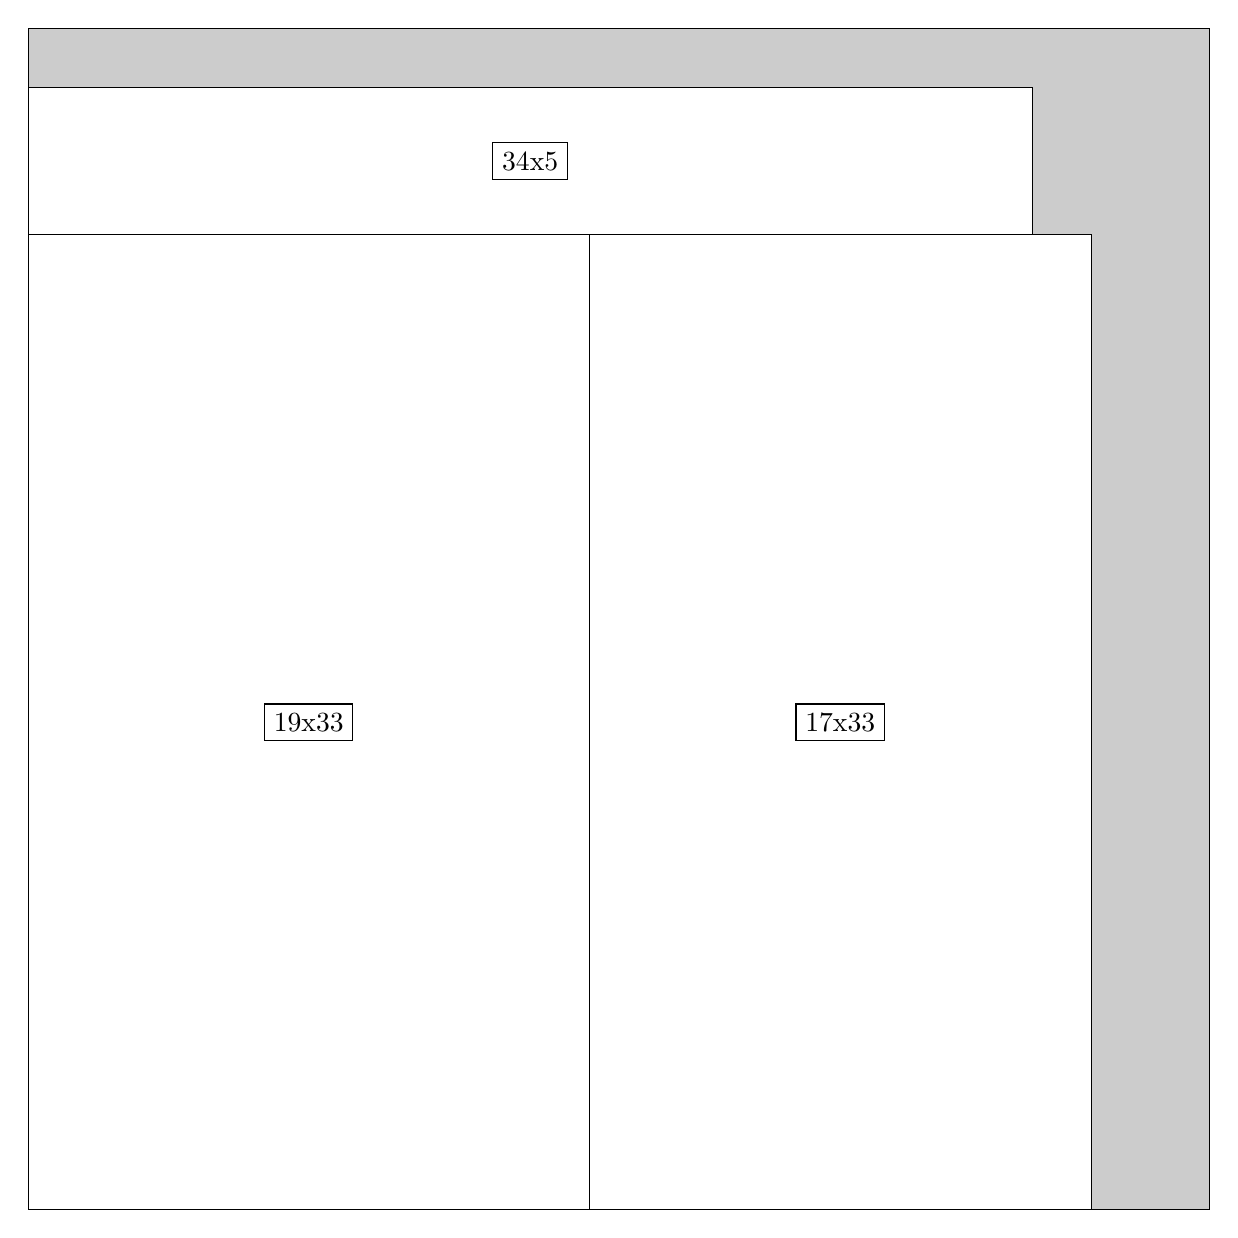
\begin{tikzpicture}[shorten >=1pt,scale=1.0,every node/.style={scale=1.0},->]
\tikzstyle{vertex}=[circle,fill=black!25,minimum size=14pt,inner sep=0pt]
\filldraw[fill=gray!40!white, draw=black] (0,0) rectangle (15.0,15.0);
\foreach \name/\x/\y/\w/\h in {19x33/0.0/0.0/7.125/12.375,17x33/7.125/0.0/6.375/12.375,34x5/0.0/12.375/12.75/1.875}
\filldraw[fill=white!40!white, draw=black] (\x,\y) rectangle node[draw] (\name) {\name} ++(\w,\h);
\end{tikzpicture}


w =19 , h =33 , x =0 , y =0 , v =627
\par
w =17 , h =33 , x =19 , y =0 , v =561
\par
w =34 , h =5 , x =0 , y =33 , v =170
\par
\newpage


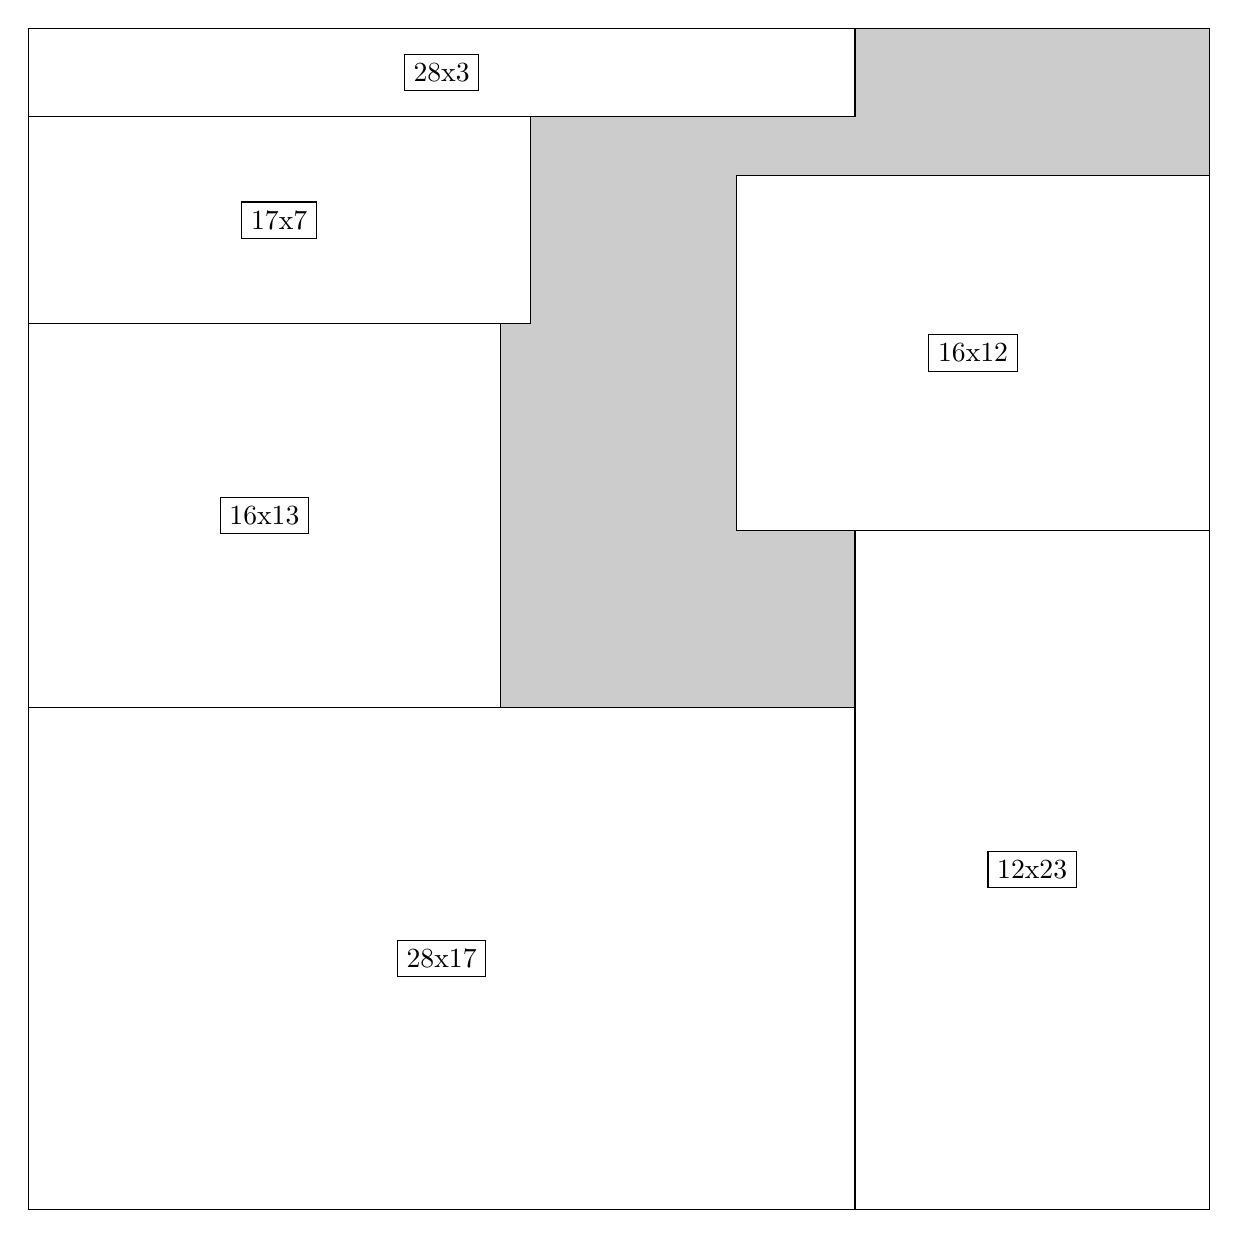
\begin{tikzpicture}[shorten >=1pt,scale=1.0,every node/.style={scale=1.0},->]
\tikzstyle{vertex}=[circle,fill=black!25,minimum size=14pt,inner sep=0pt]
\filldraw[fill=gray!40!white, draw=black] (0,0) rectangle (15.0,15.0);
\foreach \name/\x/\y/\w/\h in {28x17/0.0/0.0/10.5/6.375,12x23/10.5/0.0/4.5/8.625,16x13/0.0/6.375/6.0/4.875,16x12/9.0/8.625/6.0/4.5,17x7/0.0/11.25/6.375/2.625,28x3/0.0/13.875/10.5/1.125}
\filldraw[fill=white!40!white, draw=black] (\x,\y) rectangle node[draw] (\name) {\name} ++(\w,\h);
\end{tikzpicture}


w =28 , h =17 , x =0 , y =0 , v =476
\par
w =12 , h =23 , x =28 , y =0 , v =276
\par
w =16 , h =13 , x =0 , y =17 , v =208
\par
w =16 , h =12 , x =24 , y =23 , v =192
\par
w =17 , h =7 , x =0 , y =30 , v =119
\par
w =28 , h =3 , x =0 , y =37 , v =84
\par
\newpage


\end{document}